\documentclass[]{article}
\usepackage{mathrsfs}
\usepackage{amsfonts}
\usepackage{graphicx}


\begin{document}
\huge Transformada de Laplace.
\\

\normalsize Para comenzar a entender la transformada de Laplace debemos tener en claro como funciona la transformada de Fourier. Recordemos la definición.
\\
La transformada de Fourier de una función $f(t)$ se define:
$$
F(\omega) = \int_{-\infty}^{\infty}f(t)e^{-i\omega t} dt 
$$
\\
La transformada de Fourier venía acompañada de una condición necesaria que decía que $f(t)$ debe ser seccionalmente continua y de módulo integrable en todo el eje real, por ello muchas funciones no eran transformables ya que el area encerrada bajo la curva de estás tendería a infinito cuando $t\rightarrow \infty$.

Para solucionar esto, es conveniente multiplicar por un factor exponencial decreciente $e^{-\alpha t }$ obteniendose:
$$
\int_{-\infty}^{\infty} f(t) \cdot  e^{-\alpha t}\cdot  e^{-i\omega t}dt =
\int_{-\infty}^{\infty} f(t) \cdot  e^{-st}
$$
con $s=\alpha + i \hspace{3pt} \omega $
\\ Y esta es la definición de la Transformada de Laplace.
\\ Dentro del enfoque de la materia se trabajará con la versión unilateral de la transformada bajo la supocisión que todas las funciones $f(t)$ trabajadas cumpliran 
$f(t) = 0  \hspace{10pt} \forall t < 0$.
$$
F(s) = \int_{0}^{\infty} f(t) e^{-st} dt
$$

\large Teorema de existencia.
\\

\normalsize Sea $f(t)$ una función seccionalmente continua y $f(t)$ de orden exponencial $\gamma$ para $t > N \Rightarrow \exists \hspace{5pt} \mathscr{L}[f(t)]$

Una función $f(t)$ es de orden exponencial $\gamma \Longleftrightarrow$ ${\exists \hspace{5pt} M,\gamma \in \mathbb{R}  / \forall t > N: |e^{-\gamma t} f(t)| < M }$ si $t \rightarrow \infty$.

Es decir, la función en módulo no puede crecer mas que $Me^{\gamma t}$ a partir de un cierto valor $N$.


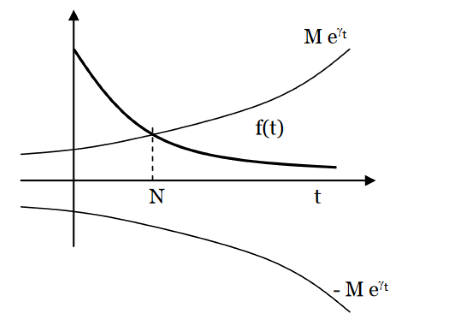
\includegraphics{../../../Imagenes/Superior/Superior01.PNG}

\large Propiedades de la transformada de Laplace
\normalsize
\\
\\
$a)$ Linealidad
$$
F(s) = \mathscr{L}[f(t)]\hspace{7pt} \wedge\hspace{7pt} G(s) = \mathscr{L}[g(t)]\hspace{7pt} \wedge\hspace{7pt} k_{1} , k_{2} \in \mathbb{R} \Rightarrow \mathscr{L}[k_{1}f(t) + k_{2}g(t)] = k_{1} F(s) + k_{2} G(s)
$$




\end{document}